\chapter{Análise de requisitos}
\minitoc
\label{chap:requisitos}
\vspace{0.5cm}

%%%%%%%%%%%%%%%%%%%%%%%%%%%%%%%%%%%%%%%%%%%%%%%%%%%%%%%%%%%%%%%%%%%%%%%%%%%%%%%%
% Objetivo: Exponer el análisis de requisitos del PFC.                         %
%%%%%%%%%%%%%%%%%%%%%%%%%%%%%%%%%%%%%%%%%%%%%%%%%%%%%%%%%%%%%%%%%%%%%%%%%%%%%%%%

\lettrine{N}{este} capítulo exporase a análise de requisitos do proxecto
baseándose no esquema proporcionado pola planificación inicial: desde a
extracción e validación de requisitos ata a realización dunha enquisa entre os
posibles usuarios, pasando por un segundo prototipo.

\section{Determinación}

 \subsection{Obxectivos}

 Establecéronse os obxectivos da fase de análise de requisitos do proxecto. \\

 Obxectivos:

 \begin{itemize}
  \item Determinar os requisitos necesarios do deseño e implementación dunha
        gaita MIDI sen fíos en tempo real empregando software/hardware libre.
 \end{itemize}

 \subsection{Alternativas}

 Establecéronse posibles alternativas a eses obxectivos, aplicables no caso de
 que estes non se puidesen cumprir. \\

 Alternativas:

 \begin{itemize}
  \item Se non é posible determinar os requisitos do proxecto, pode optarse
        por:
        \begin{enumerate}
         \item Determinar soamente os requisitos daquelas partes que sexa
               posible.
         \item Cancelar e mudar de proxecto.
        \end{enumerate}
 \end{itemize}

 \subsection{Restriccións}

 Establecéronse restriccións aplicables a ditos obxectivos.

 \begin{itemize}
  \item As propias restriccións veñen dadas polo propio título do proxecto. A
        saber:
        \begin{enumerate}
         \item Empregar o protocolo MIDI.
         \item Empregar tecnoloxía sen fíos.
         \item Empregar tempo real.
         \item Empregar software libre.
         \item Empregar harwdware libre.
         \item E/ou as derivadas de calquera das súas alternativas.
        \end{enumerate}
 \end{itemize}

\section{Avaliación de alternativas e resolución de riscos}

 \subsection{Análise de riscos}

 Determináronse os riscos que comportaban as distintas alternativas e as súas
 posibles solucións.

 \begin{itemize}
  \item Alternativas 1.
        \begin{enumerate}
         \item Riscos:
               \begin{enumerate}
                \item Que nin a posteriori se poidan obter os requisitos das
                      partes restantes.
                \item Que os requisitos obtidos a posteriori:
                      \begin{enumerate}
                       \item Eleven moito os custes temporais, económicos, de
                             es esforzo e/ou de recursos.
                       \item Sexan incompatibles cos xa obtidos.
                      \end{enumerate}
                \item Que o tempo restante para a execución do proxecto non
                      sexa suficiente.
               \end{enumerate}
         \item Solucións:
               \begin{enumerate}
                \item Aplicar algunha das subsolucións alternativas ou cancelar
                      e mudar de proxecto.
                \item Solucións propostas:
                      \begin{enumerate}
                       \item Aplicar medidas de mitigación para que a
                             planificación non se vexa afectada en extremo, ou
                             cancelar e mudar de proxecto se fan inviable o
                             mesmo.
                       \item Reanalizar os requisitos e refactorizar os mesmos
                             ata obter un sistema compatible, ou cancelar e
                             mudar de proxecto se non é posible.
                      \end{enumerate}
                \item Agardar a presentalo na seguinte convocatoria.
               \end{enumerate}
        \end{enumerate}
 \end{itemize}

 \subsection{Prototipo 2}

 Como segundo prototipo optouse por realizar unha interface gráfica
 semi-funcional de desenvolvemento rápido que plasmara os requisitos básicos
 típicos de sistemas similares xa existentes coa fin de avaliar os mesmos e
 obter novos requisitos ou desbotar parte dos xa obtidos, así como ir obtendo
 parte do deseño e distribución dos elementos da interface. \\

 A idea principal era ter algo tanxible co que tanto expertos coma outros
 usuarios puideran interactuar debido a que obter os requisitos en abstracto
 dun sistema tan complexo non é sinxelo. Ademais, a maioría das veces, tanto
 expertos coma usuarios en xeral, “non saben o que queren pero si o que non
 queren”, polo que resulta moito máis sinxelo darlles algo que poder criticar
 que dé pé tanto a desbotar requisitos xa presentes como á obtención de novos
 requisitos. \\

 Así mesmo, presentóuselles o primeiro prototipo (desenvolvido na primeira
 fase) para poder facer exactamente o mesmo cos requisitos hardware. \\

 A continuación (figuras \ref{figura:Prototipo2Inicio} a
 \ref{figura:Prototipo2Dixitacion}) preséntanse tódalas pantallas da interface
 á que se chegou mediante proceso de prototipado rápido e que foi
 posteriormente presentada ós expertos para a súa análise conxunta co
 proxectando. \\

 \begin{figure}[htbp]
  \centering
  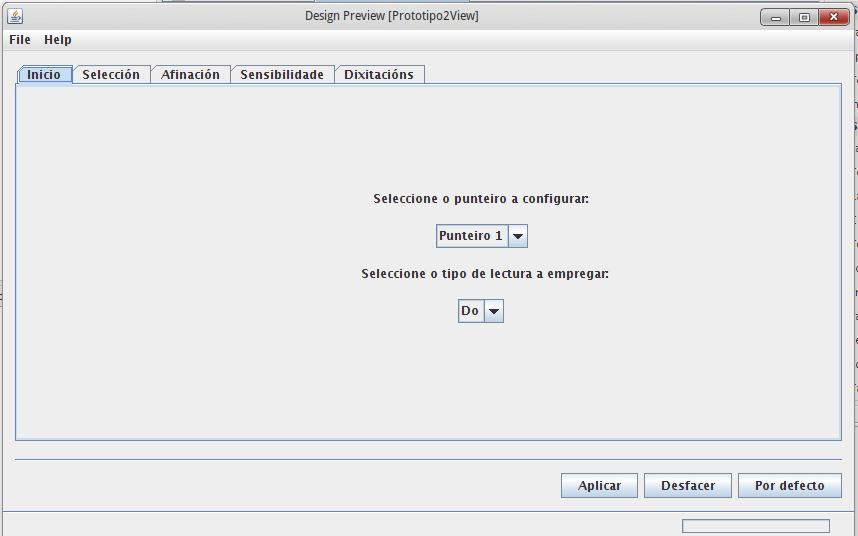
\includegraphics[scale=0.6,keepaspectratio=true]{./imagenes/prototipo2_01.png}
  % prototipo2_01.png: 858x536 pixel, 96dpi, 22.70x14.18 cm, bb=0 0 643 402
  \caption{Prototipo 2: pantalla de inicio}
  \label{figura:Prototipo2Inicio}
 \end{figure}

 \begin{figure}[htbp]
  \centering
  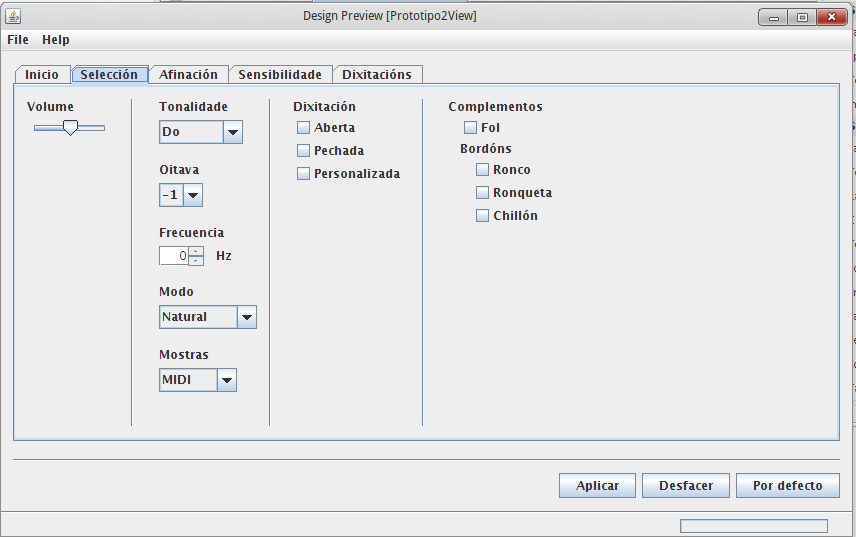
\includegraphics[scale=0.6,keepaspectratio=true]{./imagenes/prototipo2_02.png}
  % prototipo2_02.png: 856x537 pixel, 96dpi, 22.65x14.21 cm, bb=0 0 642 403
  \caption{Prototipo 2: pantalla de selección}
  \label{figura:Prototipo2Seleccion}
 \end{figure}

 \begin{figure}[htbp]
  \centering
  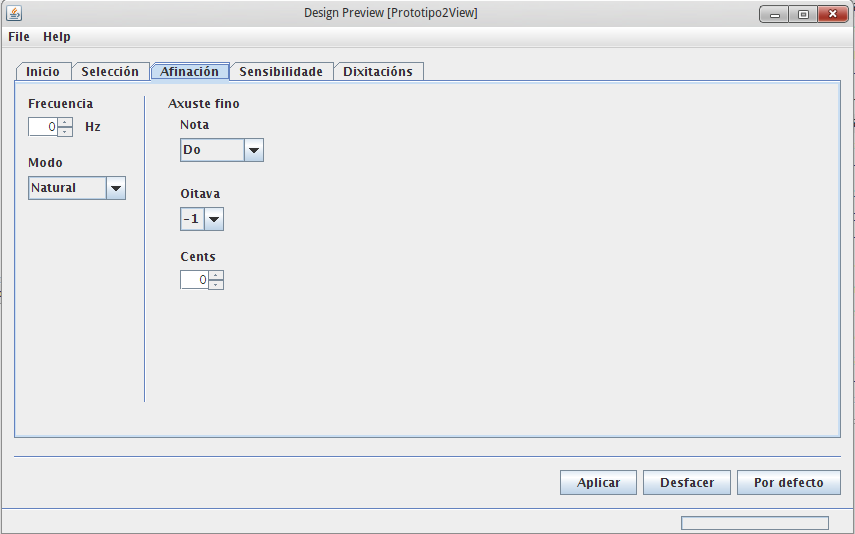
\includegraphics[scale=0.6,keepaspectratio=true]{./imagenes/prototipo2_03.png}
  % prototipo2_03.png: 855x534 pixel, 96dpi, 22.62x14.13 cm, bb=0 0 641 400
  \caption{Prototipo 2: pantalla de afinación}
  \label{figura:Prototipo2Afinacion}
 \end{figure}

 \begin{figure}[htbp]
  \centering
  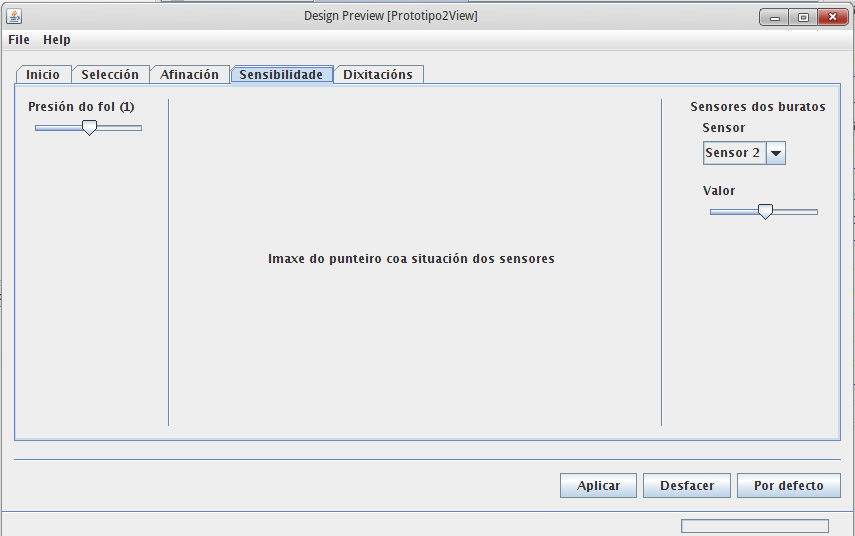
\includegraphics[scale=0.6,keepaspectratio=true]{./imagenes/prototipo2_04.png}
  % prototipo2_04.png: 855x536 pixel, 96dpi, 22.62x14.18 cm, bb=0 0 641 402
  \caption{Prototipo 2: pantalla de sensibilidade}
  \label{figura:Prototipo2Sensibilidade}
 \end{figure}

 \begin{figure}[htbp]
  \centering
  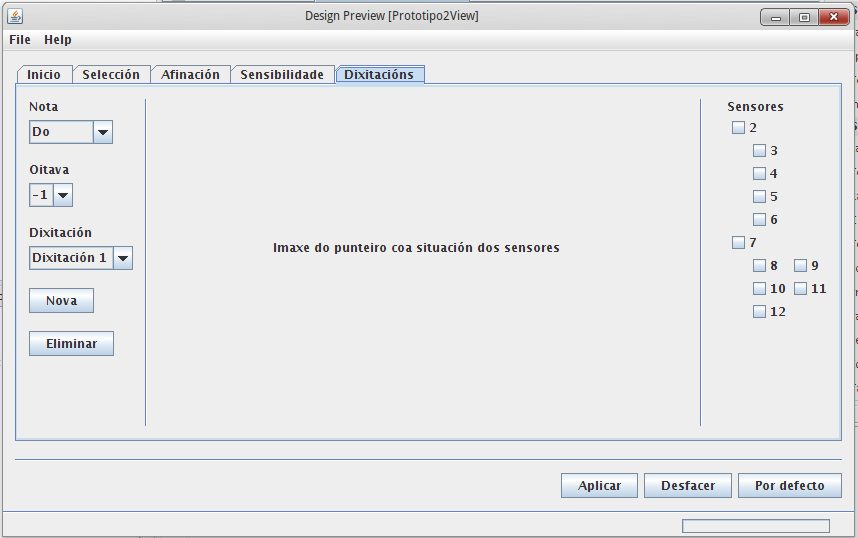
\includegraphics[scale=0.6,keepaspectratio=true]{./imagenes/prototipo2_05.png}
  % prototipo2_05.png: 858x538 pixel, 96dpi, 22.70x14.23 cm, bb=0 0 643 403
  \caption{Prototipo 2: pantalla de dixitación}
  \label{figura:Prototipo2Dixitacion}
 \end{figure}

\section{Desenvolvemento e validación do seguinte nivel do producto}

 \subsection{Simulacións, modelos e programas de proba}

 As probas a realizar neste nivel do producto consistirán en verificar sobre o
 \textit{Prototipo 2} todos aqueles requisitos software aplicables ó mesmo
 recollidos na especificación de requisitos, sendo ditas probas realizadas a
 tres bandas, é dicir, por parte do proxectando, dos expertos e de usuarios
 aleatorios.

 \subsection{Requisitos hardware, software e económicos}

  \subsubsection{Extracción de requisitos por parte do proxectando}

  Para a extracción de requisitos por parte do proxectando tivéronse en conta
  múltiples factores, xa que o obter só unha boa imitación non abonda para que
  o producto final acabe tendo éxito. Así, entre os factores que se manexaron
  destacan:

  \begin{itemize}
   \item A análise exhaustiva do equivalente ``analóxico'' e da interacción co
         usuario.
   \item A análise exhaustiva dos productos comerciais xa existentes no
         mercado.
   \item O establecemento de fortes restriccións coa fin de lograr un producto
         de calidade.
   \item A aplicación da filosofía do Software Libre.
   \item A non discriminación de usuarios.
   \item O enfoque mercantil, é dicir, o establecemento dunha estratexia
         comercial.
  \end{itemize}

  Tendo en conta estes factores e outros non menos importantes e botando man do
  \textit{Prototipo 1} e do \textit{Prototipo 2}, nos que se foron plasmando
  todas as ideas que ían surxindo, chegouse á seguinte especificación de
  requisitos software, hardware e económicos.

  \begin{itemize}
   \item \textbf{Especificación de requisitos software:}
         \begin{itemize}
          \item Principais:
                \begin{itemize}
                 \item Software libre.
                       \begin{itemize}
                        \item Todo o código desenvolvido durante o proxecto
                              será liberado baixo unha licencia libre.
                        \item Todo software que se empregue para a realización
                              do proxecto será libre  (sempre que sexa
                              posible).
                       \end{itemize}
                 \item Aplicación multiplataforma.
                       \begin{itemize}
                        \item A aplicación debe de ser portable a distintos
                              sistemas operativos.
                        \item Non debe de ser necesario recompilala manualmente
                              para o seu correcto funcionamento.
                              Non debe de ter dependencia de tecnoloxías ou
                              ferramentas que limiten a súa portabilidade.
                        \item Garantiza a uniformidade da aplicación e, polo
                              tanto, reduce a curva de aprendizaxe entre
                              plataformas.
                        \item Reduce a complexidade e os custes do proxecto.
                        \item Reduce a aparición de erros e facilita a súa
                              localización e corrección.
                       \end{itemize}
                 \item Retardo mínimo.
                       \begin{itemize}
                        \item O retardo existente entre a execución dunha nota
                              e a súa audición debe de ser imperceptible ou
                              aceptable polo usuario.
                        \item Isto implica o uso de tempo real.
                        \item Máis concretamente e, relacionándoo directamente
                              co software, esixe o uso dun sistema operativo
                              con soporte para tempo real.
                       \end{itemize}
                 \item Emprego da mesma configuración en entornos distintos.
                       \begin{itemize}
                        \item Non é de rigor ter que reconfigurar o punteiro de
                              cada vez que o queremos empregar, nin ter que
                              facelo se o empregamos nun equipo distinto ó
                              habitual.
                        \item Implica que a configuración debe ser gardada no
                              punteiro.
                       \end{itemize}
                 \item Uso de varios punteiros sobre a mesma aplicación e
                       receptor.
                       \begin{itemize}
                        \item Uso de varios punteiros sobre a mesma aplicación
                              e receptor.
                        \item Non é de rigor ter que empregar varias instancias
                              da aplicación e/ou varios equipos para poder
                              empregar varios punteiros.
                       \end{itemize}
                 \item Regulación da presión do fol.
                       \begin{itemize}
                        \item Debe de ser posible a regulación da presión
                              necesaria para facer soar o punteiro.
                        \item Non tódolos usuarios apretan o mesmo.
                       \end{itemize}
                 \item Regulación da sensibilidade dos sensores, tanto conxunta
                       coma independentemente.
                       \begin{itemize}
                        \item Non hai dúas persoas iguais e, incluso dentro da
                              mesma persoa, non tódolos dedos son iguais, polo
                              que é preciso poder regular os sensores para o
                              correcto funcionamento do punteiro.
                       \end{itemize}
                 \item Regulación de volume.
                       \begin{itemize}
                        \item Debe ser posible regular o volume de saída do
                              son, por motivos evidentes.
                       \end{itemize}
                 \item Regulación da tonalidade ou nota base.
                       \begin{itemize}
                        \item Debe ser posible tocar en calquera tonalidade sen
                              limitación algunha de nota ou altura.
                       \end{itemize}
                 \item Regulación da frecuencia base de afinación.
                       \begin{itemize}
                        \item Debe ser posible regular a frecuencia base de
                              afinación.
                        \item Dependendo da situación, é preciso afinar nunha
                              frecuencia ou noutra.
                       \end{itemize}
                 \item Regulación individual da frecuencia de afinación de cada
                       nota.
                       \begin{itemize}
                        \item Debe ser posible retocar individualmente a
                              afinación de cada nota co fin de poder afinar
                              correctamente cos bordóns “analóxicos” da gaita
                              e/ou con outros instrumentos.
                       \end{itemize}
                 \item Configuración da dixitación.
                       \begin{itemize}
                        \item Empregarase a dixitación da gaita galega (aberta,
                              pechada).
                        \item Darase a posibilidade de incluír outras
                              dixitacións ou persoalizar as xa existentes.
                       \end{itemize}
                 \item Tesitura ilimitada.
                       \begin{itemize}
                        \item A maioría das opcións comerciais existentes
                              limitan moito a tesitura, o que limita gravemente
                              ó usuario á hora de interpretar unha peza.
                        \item Debe ser o propio usuario o que decida ónde están
                              os seus límites, non o sistema.
                       \end{itemize}
                \end{itemize}
          \item Opcionais:
                \begin{itemize}
                 \item Menús navegables dende o punteiro.
                       \begin{itemize}
                        \item Facilita a tarefa de variar a configuración do
                              punteiro sen ter que achegarse á computadora.
                       \end{itemize}
                 \item Deshabilitación do sensor de presión.
                       \begin{itemize}
                        \item O sensor de presión emprégase para evaluar cándo
                              debe de soar a gaita.
                        \item Sería interesante poder facelo tamén empregando
                              unha ``dixitación especial'' que nos permitise
                              poder tocar sen ter que facer uso do fol.
                        \item Existen moitos casos nos que isto sería unha
                              opción moi cómoda.
                       \end{itemize}
                 \item ``Vibrato continuo''.
                       \begin{itemize}
                        \item Posibilidade aplicar a técnica de
                              ``vibrato continuo'' presente noutros punteiros
                              comerciais.
                       \end{itemize}
                 \item Inclusión de bordóns.
                       \begin{itemize}
                        \item Ronco, ronqueta e chillón.
                        \item Sobre afinación natural.
                        \item Con posibilidade de aplicar cortes.
                       \end{itemize}
                 \item Uso de \textit{samples} reais.
                       \begin{itemize}
                        \item Inclusión da posibilidade do uso de
                              \textit{samples} pregravados no canto de MIDI.
                        \item Posibilidade de distintas afinacións e/ou toques.
                       \end{itemize}
                \end{itemize}
         \end{itemize}
   \item \textbf{Especificación de requisitos hardware:}
         \begin{itemize}
          \item Principais:
                \begin{itemize}
                 \item Uso de hardware libre.
                       \begin{itemize}
                        \item Todo o hardware empregado na construcción do
                              punteiro ha de ser libre.
                       \end{itemize}
                 \item Punteiro ó máis parecido a un punteiro ``analóxico''.
                       \begin{itemize}
                        \item Mínima intrusión, mínimo rechazo.
                       \end{itemize}
                 \item Uso de sensores capacitivos.
                       \begin{itemize}
                        \item Son os máis adecuados.
                       \end{itemize}
                 \item Mesmas dimensións para tódolos buratos.
                       \begin{itemize}
                        \item Facilita o uso e axuste dos sensores.
                       \end{itemize}
                 \item Conexión sen fíos.
                       \begin{itemize}
                        \item Facilita a mobilidade e a comodiade á hora de
                              empregar o punteiro.
                        \item Mínima intrusión, mínimo rechazo.
                        \item Pode verse condicionada á falta de espacio no
                              punteiro, debido á necesidade de incorporar unha
                              batería recargable.
                       \end{itemize}
                \end{itemize}
          \item Opcionais:
                \begin{itemize}
                 \item Inclusión de botóns de selección.
                       \begin{itemize}
                        \item Facilita a tarefa de variar a configuración do
                              punteiro sen ter que achegarse á computadora.
                        \item Esta opción dependerá do espacio físico sobrante
                              no interior do punteiro.
                       \end{itemize}
                 \item Entrega do producto en estuche de calidade.
                       \begin{itemize}
                        \item Dar boa impresión incrementa a confianza no
                              producto.
                        \item Dependerá dos requisitos económicos.
                       \end{itemize}
                 \item Entrega dun netbook/tablet ou similar debidamente
                       preparado e configurado para empregar coa gaita.
                       \begin{itemize}
                        \item Concepto ``plug \& play''.
                        \item A día de hoxe segue existindo unha ampla cota de
                              que non está familiarizada coa informática
                              básica, polo que sería interesante ofrecer dita
                              opción.
                        \item Dependerá dos requisitos económicos.
                       \end{itemize}
                \end{itemize}
         \end{itemize}
   \item \textbf{Especificación de requisitos económicos:}
         \begin{itemize}
          \item Principais:
                \begin{itemize}
                 \item Saída ó mercado do modelo básico por debaixo dos 600
                       euros.
                       \begin{itemize}
                        \item En ningún caso debería de sobrepasar os 600
                              euros, salvo inclusión de hardware adicional
                              opcional.
                       \end{itemize}
                \end{itemize}
         \end{itemize}
  \end{itemize}

  \subsubsection{Extracción de requisitos por parte de expertos}

  Para a extracción de requisitos por parte de expertos, preseleccionáronse
  dous recoñecidos expertos na materia entre os moitos existentes e coñecidos
  por parte do proxectando. \\

  \textbf{Xosé Luis ``Lis'' Latas Vilanova}

  \begin{figure}[htbp]
   \centering
   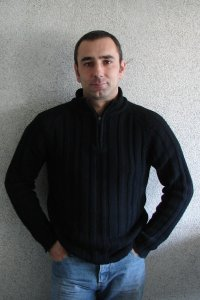
\includegraphics[keepaspectratio=true]{./imagenes/lis-latas.jpg}
   % lis-latas.jpg: 200x300 pixel, 300dpi, 1.69x2.54 cm, bb=0 0 48 72
   \caption{Lis Latas}
   \label{figura:LisLatas}
  \end{figure}

  \begin{quotation}
  \slshape

   \textit{Xosé Luís Latas Vilanova} (Lugo, 1971) \cite{LisLatas}, coñecido nos
   ambientes gaiteirís como \textit{Lis Latas}, pertence a esa nova e brillante
   xeración de artesáns en que conflúen todos os saberes e técnicas
   tradicionais de construción da gaita a carón das máis avanzadas pesquisas e
   investigacións destinadas a melloraren o instrumento nacional galego por
   excelencia. Así, após un estudo minucioso da construción, tímbrica e
   afinación das gaitas galegas antigas, pasando por unha análise rigorosa das
   súas características sonoras na época actual, as gaitas que levan o selo Lis
   posúen un timbre de seu, propio, que combina o mellor da estética sonora de
   hai tempo coa minuciosidade na afinación, capaces de singularizaren positiva
   e acusticamente os instrumentos construídos no
   \textit{Obradoiro de Gaitas Lis Latas}. E esa perfección na afinación da
   escala da gaita foi conseguida combinando variábeis fundamentais que teñen
   incidencia directa nesa cualidade sonora: por un lado, mediante o estudo
   pormenorizado da localización exacta (en décimas de milímetro) en que debe
   ir un burato do punteiro; en segundo lugar, a través da comparación do
   diámetro entre os diferentes buratos entre si, atendendo á columna de ar;
   como terceiro factor a se ter en conta, mediante unnha análise milimétrica
   das dimensións da lonxitude do punteiro; aliás, a través dunha investigación
   rigorosa da súa precisa conicidade; e, finalmente, grazas a unha minuciosa
   análise dos ouvidos que se achan na base do punteiro e da relación que
   presentan entre si. Son, pois, uns instrumentos capaces de afinaren a 440 en
   calquera das súas notas, máxime a termos en conta o punteiro afinábel,
   verdadeira carta de presentación do Obradoiro e do cal falaremos máis
   abaixo. \\

   Con 4 anos inicia as súas primeiras clases de baile tradicional en
   \textit{Candai}, na \textit{casa de Tiopedro}, continuando no grupo
   \textit{As Feiticeiras de Paradai} no que ingresa ós 7 anos de idade. Dous
   anos despois pasa a formar parte das escolas de \textit{Cántigas e Frores}
   de Lugo, onde toma os primeiros contactos coa gaita galega. Ós 14 anos
   comeza a impartir clases de baile en diferentes parbularios e, xa con 17,
   entra a formar parte da primeira asociación de mestres de baile de Lugo. Un
   ano máis tarde nace unha nova asociación cultural na capital lucense,
   \textit{Reviravolta}, da que é socio fundador. A partir deste momento comeza
   a dar clases de baile e gaita en diferentes asociacións da provincia de Lugo
   e o occidente de Asturias: \textit{Antaruxas e Sorteiros} da Fonsagrada,
   \textit{Airiños do Neira} de Baralla, \textit{Xistra} de Pedrafita do
   Cebreiro, asociación de Triacastela, \textit{Os Castros} en Taramundi,
   \textit{Pola Vila} de San Antolín de Íbias, asociación de San Martín de
   Oscos, asociación do Cádabo e tamén no colexio da mesma localidade,
   asociación de veciños de Conturiz, ... \\

   Realiza estudios universitarios na \textit{Escola de Maxisterio Infantil} do
   campus lucense. Na súa ampla traxectoria profesional forma parte de
   proxectos de diferente índole:

   \begin{itemize}
    \item Na actualidade forma parte do grupo folk \textit{Reviravolta} de Lugo
          como director musical.
    \item Traballa durante 4 anos (1996-2000) na tenda musical
          \textit{Arco Iris} de Lugo como técnico da sección de folk e
          reparador de instrumentos musicais.
    \item No ano 1997 produce o disco \textit{O Miño non pasa por Escocia} do
          grupo \textit{Reviravolta}.
    \item Colabora no disco \textit{Razas} de \textit{Arturo Vaquero} (1998).
          Participa na banda sonora da serie televisiva
          \textit{Camiño de Santiago}, emitida en Telecinco no ano 1999.
    \item Comeza no mundo da construcción de instrumentos no ano 1999 da man do
          ilustre gaiteiro, \textit{Pepe Vaamonde}, pilar fundamental na súa
          evolución como artesán.
    \item Presenta o traballo discográfico \textit{166.000 Xentes Libres} no
          \textit{Lincoln Center de Nova York} (novembro do 2000).
    \item Colabora con diferentes grupos musicais: \textit{Seare} de Sarria e
          \textit{Os moricegos de Taramundi}.
    \item Realiza un curso de ebanistería impartido polo mestre
          \textit{Delfín Blanco} no ano 2001. 
    \item No ano 2002 patenta o primeiro punteiro afinable do mundo
          incorporando unha mellora á patente no 2005.
    \item Ademais do seu traballo como artesán, na actualidade segue impartindo
          clases de baile nalgunhas asociacións da provincia lucense e
          dirixindo o grupo folk \textit{Reviravolta}.
   \end{itemize}
  \end{quotation}

  \textbf{Pepe Vaamonde Manteiga}

  \begin{figure}[htbp]
   \centering
   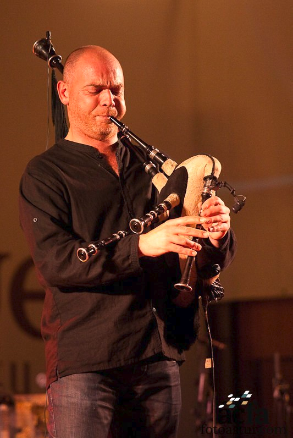
\includegraphics[scale=0.8,keepaspectratio=true]{./imagenes/pepe-vaamonde.png}
   % pepe-vaamonde.png: 293x438 pixel, 96dpi, 7.75x11.59 cm, bb=0 0 220 328
   \caption{Pepe Vaamonde}
   \label{figura:PepeVaamonde}
  \end{figure}

  \begin{quotation}
  \slshape

   Leva máis de 25 anos vinculado á gaita e á música folc. Con 15 anos empeza a
   compor e na década dos noventa gaña a maioría de concursos de Galicia como
   gaiteiro solista (\textit{I Certame Pelegrín}, \textit{Soutelo de Montes},
   tres edicións do \textit{Constantino Bellón} -o concurso máis importante a
   nivel galego-). \\

   É sobre todo un gaiteiro cun son propio, que é capaz de interpretar as
   pasaxes máis virtuosas e os máis emotivos cunha mestría inaudita. \\

   Actualmente compaxina o seu traballo en \textit{Pepe Vaamonde Grupo (PVG)}
   \cite{PVG} co seu labor docente en varias asociacións folclóricas e no
   \textit{Centro de Música Fingoi} de Lugo. \\
  \end{quotation}

  Ambos expertos traballan xuntos no obradoiro de construcción de gaitas
  \textit{Lis Latas}, feito polo cal están acostumados a colaborar entre eles e
  polo que existe certa simbiose que axudará á hora da extracción de
  requisitos. Isto, xunto cos coñecementos previo de ambos por parte do
  proxectando, axudará enormemente na comprensión entre tódalas partes e na
  chegada a bo porto do procedemento. \\

  O procedemento seguido para a extracción de requisitos por parte dos expertos
  consistiu na exposición por parte do proxectando dos requisitos previamente
  extraídos, apoiándose no \textit{Prototipo 1} e \textit{Prototipo 2}, para
  posteriormente discutilos e avalialos un por un cos expertos, dándoos finalmente
  todos por bos. Así mesmo, instouse ós expertos a avaliar se faltaba ou
  sobraba algún, dando lugar unicamente á inclusión do seguinte requisito
  hardware:

  \begin{itemize}
   \item Superficie dos sensores colocada por debaixo da zona de contacto.
         \begin{itemize}
          \item Dá sensación de burato.
          \item Facilita a adaptación e o uso do punteiro.
          \item Mínima instrusión, mínimo rechazo.
         \end{itemize}
  \end{itemize}

  \subsubsection{Extracción de requisitos por parte dos usuarios}

  Como se comentou no capítulo \ref{chap:viabilidad}, para a extracción de
  requisitos a través dos usuarios creouse unha enquisa anónima dispoñible en
  liña \cite{Enquisa} na que se preguntaba sobre datos persoais non
  identificativos (idade, procedencia), o seu perfil coma gaiteiro,
  coñecementos sobre as gaitas MIDI, caracterísiticas (fixadas de antemán en
  extraccións previas) preferibles dunha gaita MIDI e a súa prioridade,
  características propias a engadir e a súa prioridade e un pequeno estudio
  económico. A redacción da enquisa pode consultarse tamén no capítulo
  \ref{chap:viabilidad}. \\

  Como se pode observar, na enquisa non se indicaron tódolos requisitos
  extraídos anteriormente, senón que se tratou de reflexar os máis importantes
  (para dar unha idea básica das funcionalidades do producto) mesturados con
  outros non tan obvios (para poder confirmalos, aprazalos ou desbotalos).
  Ademais, non se explicou o motivo de ningún dos mesmos, para que o enquisado
  tivera que reflexionar por si mesmo o motivo da súa inclusión. E ó mesturar
  os requisitos básicos cos opcionais podíanse descartar máis facilmente
  respostas incoherentes (por exemplo, se un enquisado incluía os opcionais e
  non incluía os básicos). \\

  Así mesmo, é de facer notar que as respostas a dita enquisa non son públicas,
  polo que ningún usuario previo pode influír coas súas respostas sobre
  usuarios posteriores. Evidentemente, esta medida está enfocada a evitar un
  posible problema de falsa correlación forte nas respostas, o que podería
  invalidar totalmente a enquisa. \\

  Os resultados completos poden consultarse no apéndice \ref{chap:encuesta}. \\

  Os resultados relativos ós requisitos foron os seguintes (figuras
  \ref{figura:ResultadosExtraccionRequisitosUsuarios4} a
  \ref{figura:ResultadosExtraccionRequisitosUsuarios8}). \\

  \begin{figure}[htbp]
   \centering
   \includegraphics[scale=0.7,page=4,keepaspectratio=true]{./imagenes/enquisa.pdf}
   % enquisa.pdf: 612x792 pixel, 72dpi, 21.59x27.94 cm, bb=0 0 612 792
   \caption{Resultados da extracción de requisitos por parte dos usuarios (p. 4)}
   \label{figura:ResultadosExtraccionRequisitosUsuarios4}
  \end{figure}

  \begin{figure}[htbp]
   \centering
   \includegraphics[scale=0.7,page=5,keepaspectratio=true]{./imagenes/enquisa.pdf}
   % enquisa.pdf: 612x792 pixel, 72dpi, 21.59x27.94 cm, bb=0 0 612 792
   \caption{Resultados da extracción de requisitos por parte dos usuarios (p. 5)}
   \label{figura:ResultadosExtraccionRequisitosUsuarios5}
  \end{figure}

  \begin{figure}[htbp]
   \centering
   \includegraphics[scale=0.7,page=6,keepaspectratio=true]{./imagenes/enquisa.pdf}
   % enquisa.pdf: 612x792 pixel, 72dpi, 21.59x27.94 cm, bb=0 0 612 792
   \caption{Resultados da extracción de requisitos por parte dos usuarios (p. 6)}
   \label{figura:ResultadosExtraccionRequisitosUsuarios6}
  \end{figure}

  \begin{figure}[htbp]
   \centering
   \includegraphics[scale=0.7,page=7,keepaspectratio=true]{./imagenes/enquisa.pdf}
   % enquisa.pdf: 612x792 pixel, 72dpi, 21.59x27.94 cm, bb=0 0 612 792
   \caption{Resultados da extracción de requisitos por parte dos usuarios (p. 7)}
   \label{figura:ResultadosExtraccionRequisitosUsuarios7}
  \end{figure}

  \begin{figure}[htbp]
   \centering
   \includegraphics[scale=0.7,page=8,keepaspectratio=true]{./imagenes/enquisa.pdf}
   % enquisa.pdf: 612x792 pixel, 72dpi, 21.59x27.94 cm, bb=0 0 612 792
   \caption{Resultados da extracción de requisitos por parte dos usuarios (p. 8)}
   \label{figura:ResultadosExtraccionRequisitosUsuarios8}
  \end{figure}

  Tendo en conta estes resultados, podemos afirmar que o perfil xeral do
  gaiteiro que respondeu a enquisa:

  \begin{itemize}
   \item Comprende perfectamente a importancia da ausencia de retardos.
   \item Non ten de todo claro o porqué da salvagarda da configuración entre
         usos.
   \item Considera importante que a presión do fol sexa regulable.
   \item Considera importante a regulación independente dos sensores dos dedos
         aínda que non o ten de todo claro.
   \item Considera indispensable que a a afinación base sexa regulable.
   \item Tamén considera indispensable que dita afinación se poida regular por
         nota.
   \item A dixitación personalizable parece darlle igual, aínda que a prefire.
   \item Non ten moi claro que a posibilidade de deshabilitar o sensor do fol
         sexa un requisito esixible.
   \item Sabe que o vibrato é un requisito importante.
   \item O mesmo pasa cos glisandos, aínda que non tan claramente.
   \item Élle indiferente que teña bordóns ou non.
   \item Pide claramente uns \textit{samples} de calidade.
   \item Quere un punteiro con forma tradicional.
   \item E que dito punteiro sexa acoplable a un fol calquera.
   \item Cre indispensable que se poida conectar a un ordenador.
   \item E que esa conexión se poida realizar sen fíos de por medio.
  \end{itemize}

  Como extración de requisitos propia dos usuarios, atopámonos con tres
  peticións interesantes:

  \begin{itemize}
   \item Inclusión dunha toma para auriculares.
   \item Tesitura de dúas oitavas completas máis a sensible inferior.
   \item Idéntico tamaño e forma que un punteiro normal.
  \end{itemize}

  Todas estaban contempladas xa nos requisitos obtidos anteriormente,

  \begin{itemize}
   \item a primeira iría incluída no ordenador ou equivalente ó que se
         conectase
   \item a segunda está xa contemplada no \textit{Prototipo 2}, como se pode
         comprobar,
   \item e a terceira tamén,
  \end{itemize}

  pero pasaron a formar parte máis especificamente dos requisitos, para non
  pasalos por alto en futuras consultas da documentación. \\

  Así mesmo, resulta interesante comprobar que os posibles usuarios se tomaron
  a enquisa en serio e incluso se preocuparon por achegar posibles requisitos
  moi específicos e que non son nada fáciles de detectar a priori. \\

  E centrándose xa na parte final da enquisa, o estudio económico, conta con
  datos moi interesantes. \\

  Á hora de respostar á pregunta sobre se mercarían unha gaita MIDI coas
  caracterísiticas anteriores (incluidas as propostas polos propios usuarios)
  todos respostaron afirmativamente (incluso aqueles que albergaban dúbidas ou
  non estaban totalmente interesados), o que nos fai pensar que imos por bo
  camiño. \\

  Por este motivo, a pregunta sobre as razóns para non mercala quedou sen
  resposta. \\

  A seguinte pregunta, en conxunción coa última, estaban formuladas e ordenadas
  de maneira tal que formasen unha ``pregunta trampa'' co fin de:

  \begin{itemize}
   \item Por unha banda, saber o que estarían dispostos a pagar a cegas por un
         producto destas características.
   \item Por outra, saber o que estarían dispostos a pagar polo mesmo, dentro
         dun entorno acotado, é dicir, con información previa.
   \item E, por último e quizáis o máis importante, ser capaces de detectar
         posibles \textit{outliers} que nos puidesen levar a engano.
  \end{itemize}

  A pregunta intermedia tamén axudaba no cometido, pois conseguía distraer ó
  usuario entre unha e outra e darlle tempo para volver a pensar antes de
  responder novamente. \\

  Avaliando as respostas a ditas preguntas obtívose información moi valiosa:

  \begin{itemize}
   \item Que as respostas apenas varían dunha pregunta á outra.
   \item Que as respostas á primeira pregunta estaban xa acotadas dentro do
         intervalo exposto posteriormente.
   \item Que parecen existir dúas categorías diferenciadas con distinto centro.
         Intentando darlle explicación a dito suceso e fixándose na última
         petición de requisitos por parte dos usuarios (na que se fala do fol),
         chegouse á conclusión de que o máis probable é que os usuarios que caen
         dentro da primeira categoría (precio menor) estaban a pensar
         únicamente no punteiro e os da segunda, na gaita completa, polo que,
         sen querer, obtivéronse requisitos económicos para dúas
         configuracións distintas.
  \end{itemize}

  Centrándonos na primeira desas configuracións, actualizouse un dos requisitos
  económicos da seguinte maneira:

  \begin{itemize}
   \item Saída ó mercado do modelo básico por debaixo dos 600 euros.
         \begin{itemize}
          \item \textit{O estudio de viabilidade indica que sería aconsellable
                 que o precio estivese por debaixo dos 500 euros}.
          \item En ningún caso debería de sobrepasar os 600 euros, salvo
                inclusión de hardware adicional opcional (ver requisitos
                hardware).
         \end{itemize}
  \end{itemize}

  E volvendo á información aportada polas respostas anteriores:

  \begin{itemize}
   \item Hai un claro caso de \textit{outlier} en canto ás respostas do
         primeiro usuario no que á parte económica se refire. Con respecto á
         primeira pregunta, dá a cantidade máis alta de todas e, con respecto á
         segunda, ademais de ser a cantidade máis alta, sáese fóra do
         intervalo, o que acentúa máis se cabe a súa singularidade. Intentando
         buscarlle explicación a isto e ó mesmo tempo, saber se tiñan que
         desbotar as súas respostas, estudiamos o caso en máis profundidade. O
         resto das súas respostas non presentaban anomalías. Sen embargo, ó
         fixarse na resposta á primeira pregunta, detectamos que se trata dunha
         persoa de 14 anos, e polo tanto a priori sen experiencia en temas
         económicos, polo que é normal que as súas respostas no que a
         requisitos económicos se refire, sexan pouco acertadas. Por este
         motivo, decidiuse desbotar as súas respostas á parte económica da
         enquisa, mantendo iso si, as demáis.
  \end{itemize}

 Para rematar o apartado, volver comentar unha vez máis que dado o tamaño
 mostral o estudio resulta non significativo, pero tendo evitado o
 condicionamento entre usuarios e vista a dispersión mostral, os resultados da
 enquisa parecen amosar unha forte correlación verdadeira, motivo polo cal
 tendemos a crer que a especificación de requisitos parece acorde ó que demanda
 o mercado.

 \subsection{Validación de requisitos}

 As probas a realizar neste nivel do producto consistiron en verificar sobre os
 dous prototipos previos todos aqueles requisitos software aplicables ós mesmos
 recollidos na especificación de requisitos, verificando por parte do
 proxectando e dos expertos que o producto é correcto.

 Non se detectaron inconformidades por ningunha das partes, polo que se deu por
 correcta a especificación de requisitos, que finalmente quedou como segue:

 \begin{itemize}
   \item \textbf{Especificación de requisitos software:}
         \begin{itemize}
          \item Principais:
                \begin{itemize}
                 \item Software libre.
                       \begin{itemize}
                        \item Todo o código desenvolvido durante o proxecto
                              será liberado baixo unha licencia libre.
                        \item Todo software que se empregue para a realización
                              do proxecto será libre  (sempre que sexa
                              posible).
                       \end{itemize}
                 \item Aplicación multiplataforma.
                       \begin{itemize}
                        \item A aplicación debe de ser portable a distintos
                              sistemas operativos.
                        \item Non debe de ser necesario recompilala manualmente
                              para o seu correcto funcionamento.
                              Non debe de ter dependencia de tecnoloxías ou
                              ferramentas que limiten a súa portabilidade.
                        \item Garantiza a uniformidade da aplicación e, polo
                              tanto, reduce a curva de aprendizaxe entre
                              plataformas.
                        \item Reduce a complexidade e os custes do proxecto.
                        \item Reduce a aparición de erros e facilita a súa
                              localización e corrección.
                       \end{itemize}
                 \item Retardo mínimo.
                       \begin{itemize}
                        \item O retardo existente entre a execución dunha nota
                              e a súa audición debe de ser imperceptible ou
                              aceptable polo usuario.
                        \item Isto implica o uso de tempo real.
                        \item Máis concretamente e, relacionándoo directamente
                              co software, esixe o uso dun sistema operativo
                              con soporte para tempo real.
                       \end{itemize}
                 \item Emprego da mesma configuración en entornos distintos.
                       \begin{itemize}
                        \item Non é de rigor ter que reconfigurar o punteiro de
                              cada vez que o queremos empregar, nin ter que
                              facelo se o empregamos nun equipo distinto ó
                              habitual.
                        \item Implica que a configuración debe ser gardada no
                              punteiro.
                       \end{itemize}
                 \item Uso de varios punteiros sobre a mesma aplicación e
                       receptor.
                       \begin{itemize}
                        \item Uso de varios punteiros sobre a mesma aplicación
                              e receptor.
                        \item Non é de rigor ter que empregar varias instancias
                              da aplicación e/ou varios equipos para poder
                              empregar varios punteiros.
                       \end{itemize}
                 \item Regulación da presión do fol.
                       \begin{itemize}
                        \item Debe de ser posible a regulación da presión
                              necesaria para facer soar o punteiro.
                        \item Non tódolos usuarios apretan o mesmo.
                       \end{itemize}
                 \item Regulación da sensibilidade dos sensores, tanto conxunta
                       coma independentemente.
                       \begin{itemize}
                        \item Non hai dúas persoas iguais e, incluso dentro da
                              mesma persoa, non tódolos dedos son iguais, polo
                              que é preciso poder regular os sensores para o
                              correcto funcionamento do punteiro.
                       \end{itemize}
                 \item Regulación de volume.
                       \begin{itemize}
                        \item Debe ser posible regular o volume de saída do
                              son, por motivos evidentes.
                       \end{itemize}
                 \item Regulación da tonalidade ou nota base.
                       \begin{itemize}
                        \item Debe ser posible tocar en calquera tonalidade sen
                              limitación algunha de nota ou altura.
                       \end{itemize}
                 \item Regulación da frecuencia base de afinación.
                       \begin{itemize}
                        \item Debe ser posible regular a frecuencia base de
                              afinación.
                        \item Dependendo da situación, é preciso afinar nunha
                              frecuencia ou noutra.
                       \end{itemize}
                 \item Regulación individual da frecuencia de afinación de cada
                       nota.
                       \begin{itemize}
                        \item Debe ser posible retocar individualmente a
                              afinación de cada nota co fin de poder afinar
                              correctamente cos bordóns “analóxicos” da gaita
                              e/ou con outros instrumentos.
                       \end{itemize}
                 \item Configuración da dixitación.
                       \begin{itemize}
                        \item Empregarase a dixitación da gaita galega (aberta,
                              pechada).
                        \item Darase a posibilidade de incluír outras
                              dixitacións ou persoalizar as xa existentes.
                       \end{itemize}
                 \item Tesitura ilimitada.
                       \begin{itemize}
                        \item Alomenos dúas oitavas completas máis a sensible
                              inferior.
                        \item A maioría das opcións comerciais existentes
                              limitan moito a tesitura, o que limita gravemente
                              ó usuario á hora de interpretar unha peza.
                        \item Debe ser o propio usuario o que decida ónde están
                              os seus límites, non o sistema.
                       \end{itemize}
                \end{itemize}
          \item Opcionais:
                \begin{itemize}
                 \item Menús navegables dende o punteiro.
                       \begin{itemize}
                        \item Facilita a tarefa de variar a configuración do
                              punteiro sen ter que achegarse á computadora.
                       \end{itemize}
                 \item Deshabilitación do sensor de presión.
                       \begin{itemize}
                        \item O sensor de presión emprégase para evaluar cándo
                              debe de soar a gaita.
                        \item Sería interesante poder facelo tamén empregando
                              unha ``dixitación especial'' que nos permitise
                              poder tocar sen ter que facer uso do fol.
                        \item Existen moitos casos nos que isto sería unha
                              opción moi cómoda.
                       \end{itemize}
                 \item ``Vibrato continuo''.
                       \begin{itemize}
                        \item Posibilidade aplicar a técnica de
                              ``vibrato continuo'' presente noutros punteiros
                              comerciais.
                       \end{itemize}
                 \item Inclusión de bordóns.
                       \begin{itemize}
                        \item Ronco, ronqueta e chillón.
                        \item Sobre afinación natural.
                        \item Con posibilidade de aplicar cortes.
                       \end{itemize}
                 \item Uso de \textit{samples} reais.
                       \begin{itemize}
                        \item Inclusión da posibilidade do uso de
                              \textit{samples} pregravados no canto de MIDI.
                        \item Posibilidade de distintas afinacións e/ou toques.
                       \end{itemize}
                \end{itemize}
         \end{itemize}
   \item \textbf{Especificación de requisitos hardware:}
         \begin{itemize}
          \item Principais:
                \begin{itemize}
                 \item Uso de hardware libre.
                       \begin{itemize}
                        \item Todo o hardware empregado na construcción do
                              punteiro ha de ser libre.
                       \end{itemize}
                 \item Punteiro ó máis parecido a un punteiro ``analóxico''.
                       \begin{itemize}
                        \item Mínima intrusión, mínimo rechazo.
                       \end{itemize}
                 \item Uso de sensores capacitivos.
                       \begin{itemize}
                        \item Son os máis adecuados.
                       \end{itemize}
                 \item Mesmas dimensións para tódolos buratos.
                       \begin{itemize}
                        \item Facilita o uso e axuste dos sensores.
                       \end{itemize}
                 \item Conexión sen fíos.
                       \begin{itemize}
                        \item Facilita a mobilidade e a comodiade á hora de
                              empregar o punteiro.
                        \item Mínima intrusión, mínimo rechazo.
                        \item Pode verse condicionada á falta de espacio no
                              punteiro, debido á necesidade de incorporar unha
                              batería recargable.
                       \end{itemize}
                 \item Inclusión dunha toma para auriculares.
                       \begin{itemize}
                        \item Debe permitírselle ó usuario poder tocar e
                              escoitarse sen ter por qué causar molestias ó
                              resto de persoas ó seu arredor.
                        \item Dita toma para auriculares xa debería de ir
                              incluida no soporte ó que se conecte o punteiro,
                              polo que non debería de plantexar ningún
                              problema.
                       \end{itemize}
                \end{itemize}
          \item Opcionais:
                \begin{itemize}
                 \item Inclusión de botóns de selección.
                       \begin{itemize}
                        \item Facilita a tarefa de variar a configuración do
                              punteiro sen ter que achegarse á computadora.
                        \item Esta opción dependerá do espacio físico sobrante
                              no interior do punteiro.
                       \end{itemize}
                 \item Entrega do producto en estuche de calidade.
                       \begin{itemize}
                        \item Dar boa impresión incrementa a confianza no
                              producto.
                        \item Dependerá dos requisitos económicos.
                       \end{itemize}
                 \item Entrega dun netbook/tablet ou similar debidamente
                       preparado e configurado para empregar coa gaita.
                       \begin{itemize}
                        \item Concepto ``plug \& play''.
                        \item A día de hoxe segue existindo unha ampla cota de
                              que non está familiarizada coa informática
                              básica, polo que sería interesante ofrecer dita
                              opción.
                        \item Dependerá dos requisitos económicos.
                       \end{itemize}
                \end{itemize}
         \end{itemize}
   \item \textbf{Especificación de requisitos económicos:}
         \begin{itemize}
          \item Principais:
                \begin{itemize}
                 \item Saída ó mercado do modelo básico por debaixo dos 600
                       euros.
                       \begin{itemize}
                        \item O estudio de viabilidade indica que sería
                              aconsellable que o precio estivese por debaixo
                              dos 500 euros.
                        \item En ningún caso debería de sobrepasar os 600
                              euros, salvo inclusión de hardware adicional
                              opcional.
                       \end{itemize}
                \end{itemize}
         \end{itemize}
  \end{itemize}

\section{Planificación da próxima fase ou ciclo}

 \subsection{Planificación do deseño}

 A continuación (figura \ref{figura:PlanificacionInicialDeseno}) exponse a
 planificación inicial do ciclo de deseño. \\

 \begin{figure}[htbp]
  \centering
  %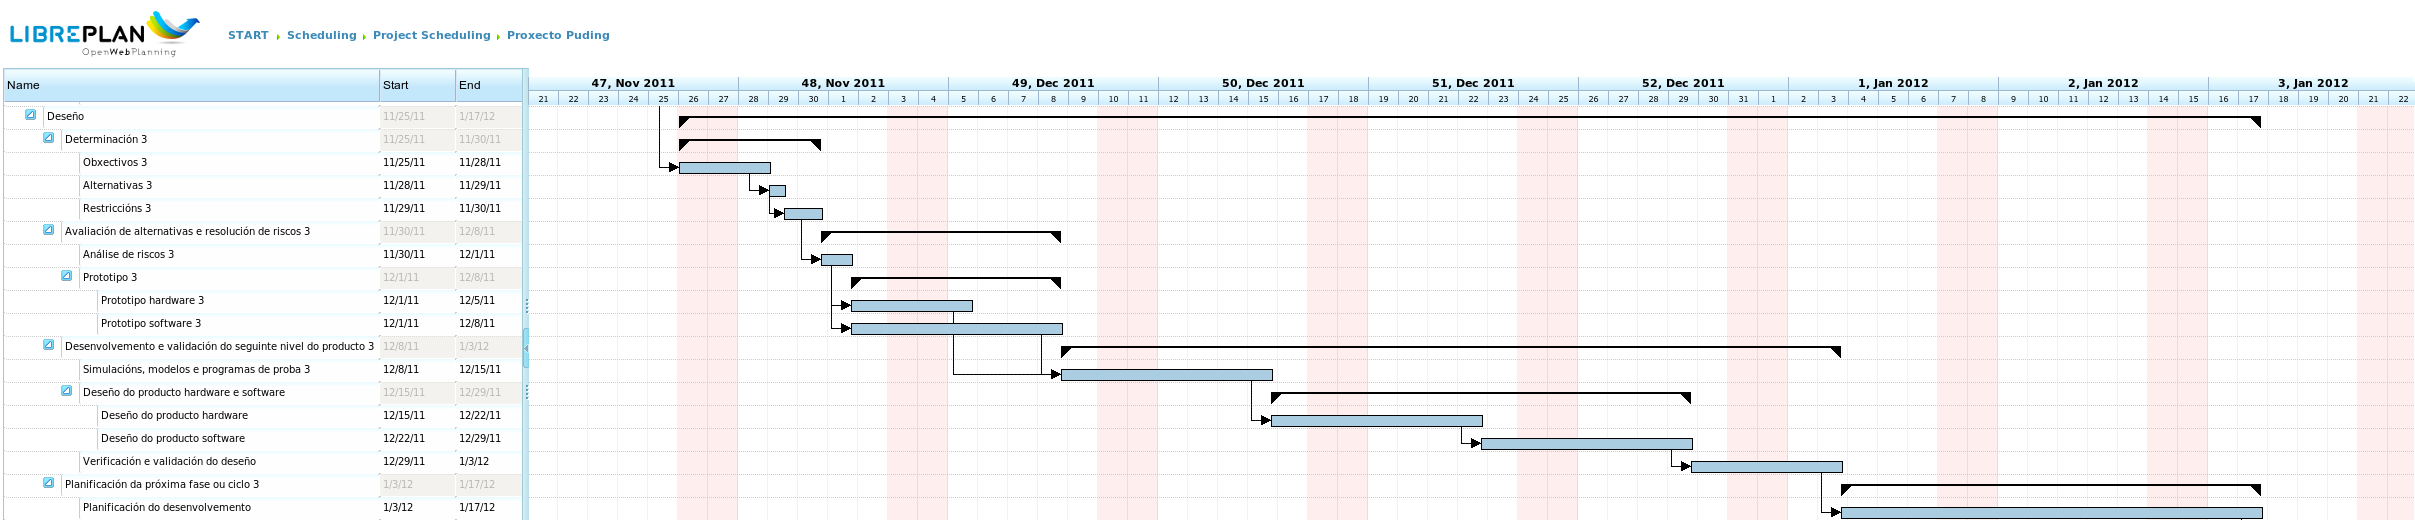
\includegraphics[scale=0.3,angle=90,keepaspectratio=true]{./imagenes/deseno.png}
  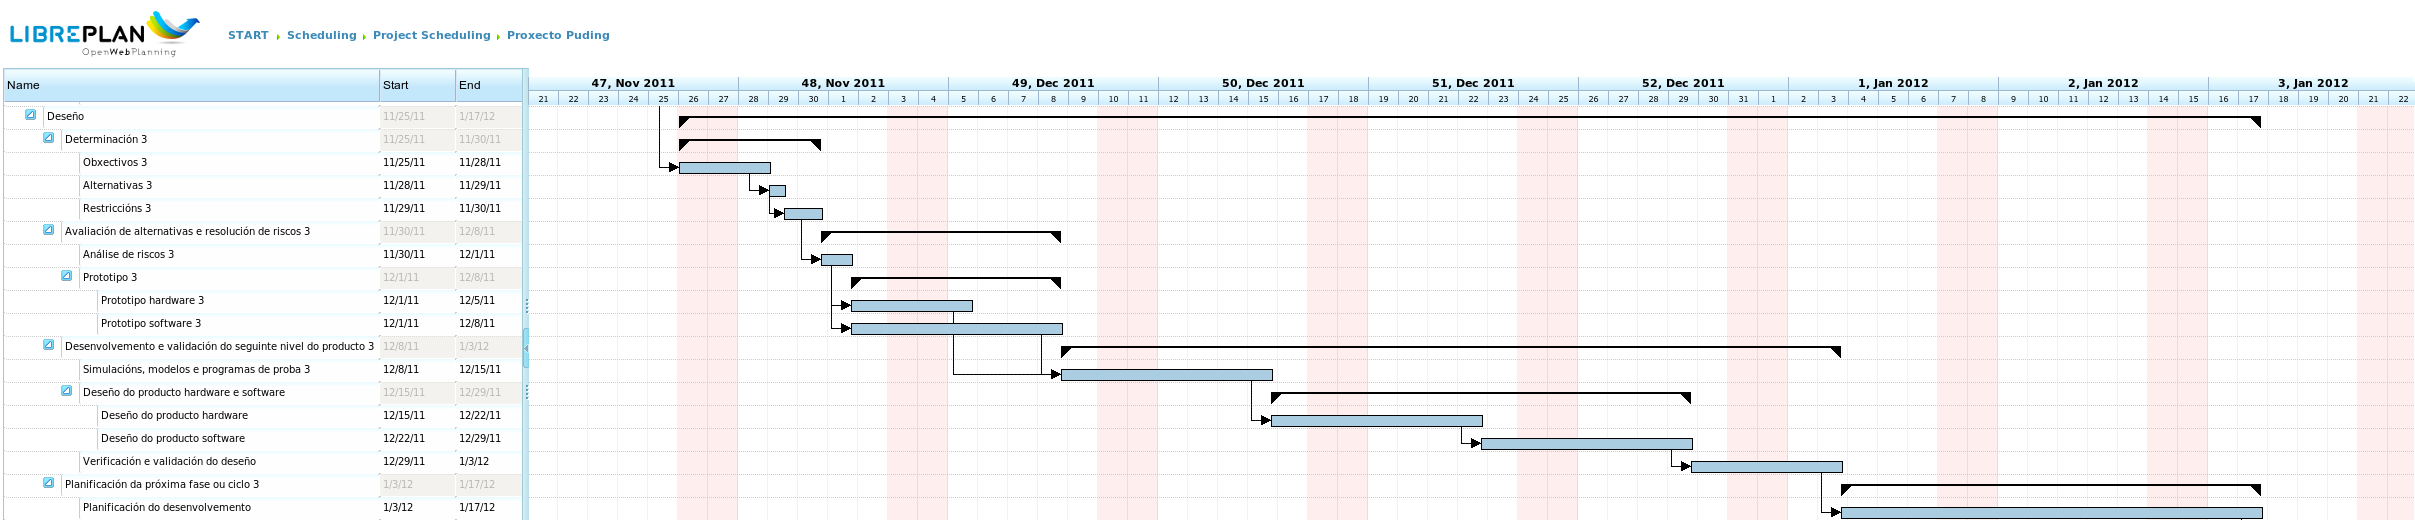
\includegraphics[trim=0 0 48cm 0,clip=true,scale=0.7,keepaspectratio=true]{./imagenes/deseno.png}
  % deseno.png: 2415x520 pixel, 100dpi, 61.34x13.21 cm, bb=0 0 1739 374
  \caption{Planificación inicial do ciclo de deseño}
  \label{figura:PlanificacionInicialDeseno}
 \end{figure}

 \textbf{Total:} 148 horas.